\documentclass[11pt]{article}
\usepackage[margin=1in]{geometry}
\usepackage[T1]{fontenc}
\usepackage{lmodern}
\usepackage{microtype}
\usepackage{booktabs}
\usepackage{graphicx}
\usepackage{hyperref}
\usepackage{xcolor}
\hypersetup{colorlinks=true,linkcolor=black,citecolor=black,urlcolor=blue!50!black}
\newcommand{\MainBmOneAcc}{64.2}
\newcommand{\MainBmOneLo}{58.2}
\newcommand{\MainBmOneHi}{69.8}
\newcommand{\MainBmOneStale}{2.3}
\newcommand{\MainBmOneAbst}{29.1}
\newcommand{\MainBmOneCtx}{961}
\newcommand{\MainBmOneMs}{6.4}
\newcommand{\MainBmOneAbstention}{95}
\newcommand{\MainBmOneAggregate}{28}
\newcommand{\MainBmOneMultihop}{0}
\newcommand{\MainBmOneSingle}{90}
\newcommand{\MainBmOneTemporal}{89}
\newcommand{\MainBmOneUpdate}{94}
\newcommand{\MainBmTwoAcc}{70.4}
\newcommand{\MainBmTwoLo}{64.6}
\newcommand{\MainBmTwoHi}{75.7}
\newcommand{\MainBmTwoStale}{1.1}
\newcommand{\MainBmTwoAbst}{25.7}
\newcommand{\MainBmTwoCtx}{1895}
\newcommand{\MainBmTwoMs}{7.1}
\newcommand{\MainBmTwoAbstention}{100}
\newcommand{\MainBmTwoAggregate}{52}
\newcommand{\MainBmTwoMultihop}{3}
\newcommand{\MainBmTwoSingle}{96}
\newcommand{\MainBmTwoTemporal}{100}
\newcommand{\MainBmTwoUpdate}{96}
\newcommand{\MainBmFourAcc}{77.0}
\newcommand{\MainBmFourLo}{71.5}
\newcommand{\MainBmFourHi}{81.8}
\newcommand{\MainBmFourStale}{1.1}
\newcommand{\MainBmFourAbst}{23.2}
\newcommand{\MainBmFourCtx}{3457}
\newcommand{\MainBmFourMs}{0.9}
\newcommand{\MainBmFourAbstention}{95}
\newcommand{\MainBmFourAggregate}{92}
\newcommand{\MainBmFourMultihop}{10}
\newcommand{\MainBmFourSingle}{100}
\newcommand{\MainBmFourTemporal}{100}
\newcommand{\MainBmFourUpdate}{99}
\newcommand{\MainBmEightAcc}{79.0}
\newcommand{\MainBmEightLo}{73.6}
\newcommand{\MainBmEightHi}{83.5}
\newcommand{\MainBmEightStale}{1.1}
\newcommand{\MainBmEightAbst}{20.7}
\newcommand{\MainBmEightCtx}{4976}
\newcommand{\MainBmEightMs}{3.0}
\newcommand{\MainBmEightAbstention}{95}
\newcommand{\MainBmEightAggregate}{92}
\newcommand{\MainBmEightMultihop}{20}
\newcommand{\MainBmEightSingle}{100}
\newcommand{\MainBmEightTemporal}{100}
\newcommand{\MainBmEightUpdate}{98}
\newcommand{\MainCardsVoneFourAcc}{88.3}
\newcommand{\MainCardsVoneFourLo}{83.8}
\newcommand{\MainCardsVoneFourHi}{91.7}
\newcommand{\MainCardsVoneFourStale}{1.1}
\newcommand{\MainCardsVoneFourAbst}{10.5}
\newcommand{\MainCardsVoneFourCtx}{3641}
\newcommand{\MainCardsVoneFourMs}{3.3}
\newcommand{\MainCardsVoneFourAbstention}{95}
\newcommand{\MainCardsVoneFourAggregate}{92}
\newcommand{\MainCardsVoneFourMultihop}{69}
\newcommand{\MainCardsVoneFourSingle}{94}
\newcommand{\MainCardsVoneFourTemporal}{95}
\newcommand{\MainCardsVoneFourUpdate}{95}
\newcommand{\MainCardsOneAcc}{72.4}
\newcommand{\MainCardsOneLo}{66.6}
\newcommand{\MainCardsOneHi}{77.5}
\newcommand{\MainCardsOneStale}{13.8}
\newcommand{\MainCardsOneAbst}{14.3}
\newcommand{\MainCardsOneCtx}{946}
\newcommand{\MainCardsOneMs}{23.1}
\newcommand{\MainCardsOneAbstention}{95}
\newcommand{\MainCardsOneAggregate}{44}
\newcommand{\MainCardsOneMultihop}{52}
\newcommand{\MainCardsOneSingle}{88}
\newcommand{\MainCardsOneTemporal}{89}
\newcommand{\MainCardsOneUpdate}{77}
\newcommand{\MainCardsTwoAcc}{84.4}
\newcommand{\MainCardsTwoLo}{79.5}
\newcommand{\MainCardsTwoHi}{88.4}
\newcommand{\MainCardsTwoStale}{8.0}
\newcommand{\MainCardsTwoAbst}{9.3}
\newcommand{\MainCardsTwoCtx}{1903}
\newcommand{\MainCardsTwoMs}{20.0}
\newcommand{\MainCardsTwoAbstention}{95}
\newcommand{\MainCardsTwoAggregate}{84}
\newcommand{\MainCardsTwoMultihop}{62}
\newcommand{\MainCardsTwoSingle}{92}
\newcommand{\MainCardsTwoTemporal}{95}
\newcommand{\MainCardsTwoUpdate}{92}
\newcommand{\MainCardsFourAcc}{89.5}
\newcommand{\MainCardsFourLo}{85.1}
\newcommand{\MainCardsFourHi}{92.7}
\newcommand{\MainCardsFourStale}{1.1}
\newcommand{\MainCardsFourAbst}{9.3}
\newcommand{\MainCardsFourCtx}{3641}
\newcommand{\MainCardsFourMs}{4.8}
\newcommand{\MainCardsFourAbstention}{95}
\newcommand{\MainCardsFourAggregate}{92}
\newcommand{\MainCardsFourMultihop}{70}
\newcommand{\MainCardsFourSingle}{98}
\newcommand{\MainCardsFourTemporal}{100}
\newcommand{\MainCardsFourUpdate}{94}
\newcommand{\MainN}{257}
\newcommand{\MainCardsEightAcc}{91.4}
\newcommand{\MainCardsEightLo}{87.4}
\newcommand{\MainCardsEightHi}{94.3}
\newcommand{\MainCardsEightStale}{1.1}
\newcommand{\MainCardsEightAbst}{7.6}
\newcommand{\MainCardsEightCtx}{6089}
\newcommand{\MainCardsEightMs}{15.6}
\newcommand{\MainCardsEightAbstention}{100}
\newcommand{\MainCardsEightAggregate}{92}
\newcommand{\MainCardsEightMultihop}{75}
\newcommand{\MainCardsEightSingle}{98}
\newcommand{\MainCardsEightTemporal}{100}
\newcommand{\MainCardsEightUpdate}{95}
\newcommand{\MainGrepFourAcc}{73.5}
\newcommand{\MainGrepFourLo}{67.8}
\newcommand{\MainGrepFourHi}{78.6}
\newcommand{\MainGrepFourStale}{0.0}
\newcommand{\MainGrepFourAbst}{26.6}
\newcommand{\MainGrepFourCtx}{3648}
\newcommand{\MainGrepFourMs}{2.7}
\newcommand{\MainGrepFourAbstention}{95}
\newcommand{\MainGrepFourAggregate}{84}
\newcommand{\MainGrepFourMultihop}{3}
\newcommand{\MainGrepFourSingle}{94}
\newcommand{\MainGrepFourTemporal}{100}
\newcommand{\MainGrepFourUpdate}{99}
\newcommand{\MainHybridFourAcc}{79.8}
\newcommand{\MainHybridFourLo}{74.4}
\newcommand{\MainHybridFourHi}{84.2}
\newcommand{\MainHybridFourStale}{0.0}
\newcommand{\MainHybridFourAbst}{21.5}
\newcommand{\MainHybridFourCtx}{3922}
\newcommand{\MainHybridFourMs}{22.0}
\newcommand{\MainHybridFourAbstention}{100}
\newcommand{\MainHybridFourAggregate}{96}
\newcommand{\MainHybridFourMultihop}{16}
\newcommand{\MainHybridFourSingle}{100}
\newcommand{\MainHybridFourTemporal}{100}
\newcommand{\MainHybridFourUpdate}{100}
\newcommand{\MainMemoryFourAcc}{63.0}
\newcommand{\MainMemoryFourLo}{57.0}
\newcommand{\MainMemoryFourHi}{68.7}
\newcommand{\MainMemoryFourStale}{2.3}
\newcommand{\MainMemoryFourAbst}{29.5}
\newcommand{\MainMemoryFourCtx}{4000}
\newcommand{\MainMemoryFourMs}{0.0}
\newcommand{\MainMemoryFourAbstention}{100}
\newcommand{\MainMemoryFourAggregate}{24}
\newcommand{\MainMemoryFourMultihop}{69}
\newcommand{\MainMemoryFourSingle}{47}
\newcommand{\MainMemoryFourTemporal}{63}
\newcommand{\MainMemoryFourUpdate}{71}
\newcommand{\MainNoneFourAcc}{7.8}
\newcommand{\MainNoneFourLo}{5.1}
\newcommand{\MainNoneFourHi}{11.7}
\newcommand{\MainNoneFourStale}{0.0}
\newcommand{\MainNoneFourAbst}{100.0}
\newcommand{\MainNoneFourCtx}{0}
\newcommand{\MainNoneFourMs}{0.0}
\newcommand{\MainNoneFourAbstention}{100}
\newcommand{\MainNoneFourAggregate}{0}
\newcommand{\MainNoneFourMultihop}{0}
\newcommand{\MainNoneFourSingle}{0}
\newcommand{\MainNoneFourTemporal}{0}
\newcommand{\MainNoneFourUpdate}{0}
\newcommand{\MainOracleFourAcc}{93.8}
\newcommand{\MainOracleFourLo}{90.1}
\newcommand{\MainOracleFourHi}{96.1}
\newcommand{\MainOracleFourStale}{0.0}
\newcommand{\MainOracleFourAbst}{5.1}
\newcommand{\MainOracleFourCtx}{282}
\newcommand{\MainOracleFourMs}{1.0}
\newcommand{\MainOracleFourAbstention}{100}
\newcommand{\MainOracleFourAggregate}{88}
\newcommand{\MainOracleFourMultihop}{80}
\newcommand{\MainOracleFourSingle}{98}
\newcommand{\MainOracleFourTemporal}{100}
\newcommand{\MainOracleFourUpdate}{100}
\newcommand{\MainRagOneAcc}{77.0}
\newcommand{\MainRagOneLo}{71.5}
\newcommand{\MainRagOneHi}{81.8}
\newcommand{\MainRagOneStale}{0.0}
\newcommand{\MainRagOneAbst}{23.2}
\newcommand{\MainRagOneCtx}{973}
\newcommand{\MainRagOneMs}{31.0}
\newcommand{\MainRagOneAbstention}{100}
\newcommand{\MainRagOneAggregate}{88}
\newcommand{\MainRagOneMultihop}{11}
\newcommand{\MainRagOneSingle}{98}
\newcommand{\MainRagOneTemporal}{100}
\newcommand{\MainRagOneUpdate}{99}
\newcommand{\MainRagTwoAcc}{78.6}
\newcommand{\MainRagTwoLo}{73.2}
\newcommand{\MainRagTwoHi}{83.2}
\newcommand{\MainRagTwoStale}{0.0}
\newcommand{\MainRagTwoAbst}{21.9}
\newcommand{\MainRagTwoCtx}{1954}
\newcommand{\MainRagTwoMs}{30.5}
\newcommand{\MainRagTwoAbstention}{100}
\newcommand{\MainRagTwoAggregate}{88}
\newcommand{\MainRagTwoMultihop}{16}
\newcommand{\MainRagTwoSingle}{98}
\newcommand{\MainRagTwoTemporal}{100}
\newcommand{\MainRagTwoUpdate}{100}
\newcommand{\MainRagFourAcc}{82.1}
\newcommand{\MainRagFourLo}{77.0}
\newcommand{\MainRagFourHi}{86.3}
\newcommand{\MainRagFourStale}{1.1}
\newcommand{\MainRagFourAbst}{17.7}
\newcommand{\MainRagFourCtx}{3921}
\newcommand{\MainRagFourMs}{22.8}
\newcommand{\MainRagFourAbstention}{100}
\newcommand{\MainRagFourAggregate}{88}
\newcommand{\MainRagFourMultihop}{31}
\newcommand{\MainRagFourSingle}{98}
\newcommand{\MainRagFourTemporal}{100}
\newcommand{\MainRagFourUpdate}{100}
\newcommand{\MainRagEightAcc}{89.5}
\newcommand{\MainRagEightLo}{85.1}
\newcommand{\MainRagEightHi}{92.7}
\newcommand{\MainRagEightStale}{0.0}
\newcommand{\MainRagEightAbst}{10.1}
\newcommand{\MainRagEightCtx}{7849}
\newcommand{\MainRagEightMs}{37.0}
\newcommand{\MainRagEightAbstention}{100}
\newcommand{\MainRagEightAggregate}{88}
\newcommand{\MainRagEightMultihop}{61}
\newcommand{\MainRagEightSingle}{100}
\newcommand{\MainRagEightTemporal}{100}
\newcommand{\MainRagEightUpdate}{100}
\newcommand{\MainPBmOne}{0.0020}
\newcommand{\MainPBmTwo}{0.0000}
\newcommand{\MainPBmFour}{0.0000}
\newcommand{\MainPBmEight}{0.0000}
\newcommand{\MainPCardsVoneFour}{0.1651}
\newcommand{\MainPGrepFour}{0.0000}
\newcommand{\MainPHybridFour}{0.0001}
\newcommand{\MainPMemoryFour}{0.0000}
\newcommand{\MainPNoneFour}{0.0000}
\newcommand{\MainPRagOne}{0.9268}
\newcommand{\MainPRagTwo}{0.0164}
\newcommand{\MainPRagFour}{0.0027}
\newcommand{\MainPRagEight}{0.2199}
\newcommand{\SevenBmFourAcc}{78.0}
\newcommand{\SevenBmFourLo}{72.6}
\newcommand{\SevenBmFourHi}{82.5}
\newcommand{\SevenBmFourStale}{1.1}
\newcommand{\SevenBmFourAbst}{23.4}
\newcommand{\SevenBmFourCtx}{3343}
\newcommand{\SevenBmFourMs}{1.4}
\newcommand{\SevenBmFourAbstention}{100}
\newcommand{\SevenBmFourAggregate}{100}
\newcommand{\SevenBmFourMultihop}{16}
\newcommand{\SevenBmFourSingle}{100}
\newcommand{\SevenBmFourTemporal}{93}
\newcommand{\SevenBmFourUpdate}{99}
\newcommand{\SevenCardsVoneOneAcc}{65.7}
\newcommand{\SevenCardsVoneOneLo}{59.8}
\newcommand{\SevenCardsVoneOneHi}{71.1}
\newcommand{\SevenCardsVoneOneStale}{26.6}
\newcommand{\SevenCardsVoneOneAbst}{15.2}
\newcommand{\SevenCardsVoneOneCtx}{959}
\newcommand{\SevenCardsVoneOneMs}{5.4}
\newcommand{\SevenCardsVoneOneAbstention}{100}
\newcommand{\SevenCardsVoneOneAggregate}{46}
\newcommand{\SevenCardsVoneOneMultihop}{49}
\newcommand{\SevenCardsVoneOneSingle}{72}
\newcommand{\SevenCardsVoneOneTemporal}{93}
\newcommand{\SevenCardsVoneOneUpdate}{67}
\newcommand{\SevenCardsVoneTwoAcc}{90.7}
\newcommand{\SevenCardsVoneTwoLo}{83.3}
\newcommand{\SevenCardsVoneTwoHi}{95.0}
\newcommand{\SevenCardsVoneTwoStale}{4.5}
\newcommand{\SevenCardsVoneTwoAbst}{6.2}
\newcommand{\SevenCardsVoneTwoCtx}{1917}
\newcommand{\SevenCardsVoneTwoMs}{9.5}
\newcommand{\SevenCardsVoneTwoAbstention}{0}
\newcommand{\SevenCardsVoneTwoAggregate}{0}
\newcommand{\SevenCardsVoneTwoMultihop}{0}
\newcommand{\SevenCardsVoneTwoSingle}{92}
\newcommand{\SevenCardsVoneTwoTemporal}{0}
\newcommand{\SevenCardsVoneTwoUpdate}{89}
\newcommand{\SevenCardsVoneFourAcc}{89.2}
\newcommand{\SevenCardsVoneFourLo}{84.9}
\newcommand{\SevenCardsVoneFourHi}{92.4}
\newcommand{\SevenCardsVoneFourStale}{3.2}
\newcommand{\SevenCardsVoneFourAbst}{10.2}
\newcommand{\SevenCardsVoneFourCtx}{3682}
\newcommand{\SevenCardsVoneFourMs}{2.7}
\newcommand{\SevenCardsVoneFourAbstention}{100}
\newcommand{\SevenCardsVoneFourAggregate}{96}
\newcommand{\SevenCardsVoneFourMultihop}{66}
\newcommand{\SevenCardsVoneFourSingle}{96}
\newcommand{\SevenCardsVoneFourTemporal}{100}
\newcommand{\SevenCardsVoneFourUpdate}{96}
\newcommand{\SevenCardsOneAcc}{73.9}
\newcommand{\SevenCardsOneLo}{68.3}
\newcommand{\SevenCardsOneHi}{78.8}
\newcommand{\SevenCardsOneStale}{20.2}
\newcommand{\SevenCardsOneAbst}{10.2}
\newcommand{\SevenCardsOneCtx}{952}
\newcommand{\SevenCardsOneMs}{5.2}
\newcommand{\SevenCardsOneAbstention}{100}
\newcommand{\SevenCardsOneAggregate}{46}
\newcommand{\SevenCardsOneMultihop}{50}
\newcommand{\SevenCardsOneSingle}{92}
\newcommand{\SevenCardsOneTemporal}{100}
\newcommand{\SevenCardsOneUpdate}{78}
\newcommand{\SevenCardsFourAcc}{90.7}
\newcommand{\SevenCardsFourLo}{86.6}
\newcommand{\SevenCardsFourHi}{93.6}
\newcommand{\SevenCardsFourStale}{2.1}
\newcommand{\SevenCardsFourAbst}{8.2}
\newcommand{\SevenCardsFourCtx}{3687}
\newcommand{\SevenCardsFourMs}{12.5}
\newcommand{\SevenCardsFourAbstention}{100}
\newcommand{\SevenCardsFourAggregate}{96}
\newcommand{\SevenCardsFourMultihop}{66}
\newcommand{\SevenCardsFourSingle}{100}
\newcommand{\SevenCardsFourTemporal}{93}
\newcommand{\SevenCardsFourUpdate}{100}
\newcommand{\SevenN}{268}
\newcommand{\SevenGrepFourAcc}{73.1}
\newcommand{\SevenGrepFourLo}{67.5}
\newcommand{\SevenGrepFourHi}{78.1}
\newcommand{\SevenGrepFourStale}{1.1}
\newcommand{\SevenGrepFourAbst}{27.9}
\newcommand{\SevenGrepFourCtx}{3471}
\newcommand{\SevenGrepFourMs}{4.6}
\newcommand{\SevenGrepFourAbstention}{100}
\newcommand{\SevenGrepFourAggregate}{96}
\newcommand{\SevenGrepFourMultihop}{0}
\newcommand{\SevenGrepFourSingle}{98}
\newcommand{\SevenGrepFourTemporal}{93}
\newcommand{\SevenGrepFourUpdate}{99}
\newcommand{\SevenHybridFourAcc}{79.1}
\newcommand{\SevenHybridFourLo}{73.8}
\newcommand{\SevenHybridFourHi}{83.5}
\newcommand{\SevenHybridFourStale}{0.0}
\newcommand{\SevenHybridFourAbst}{22.5}
\newcommand{\SevenHybridFourCtx}{3922}
\newcommand{\SevenHybridFourMs}{20.5}
\newcommand{\SevenHybridFourAbstention}{100}
\newcommand{\SevenHybridFourAggregate}{100}
\newcommand{\SevenHybridFourMultihop}{18}
\newcommand{\SevenHybridFourSingle}{100}
\newcommand{\SevenHybridFourTemporal}{100}
\newcommand{\SevenHybridFourUpdate}{100}
\newcommand{\SevenMemoryFourAcc}{76.1}
\newcommand{\SevenMemoryFourLo}{70.7}
\newcommand{\SevenMemoryFourHi}{80.8}
\newcommand{\SevenMemoryFourStale}{1.1}
\newcommand{\SevenMemoryFourAbst}{15.2}
\newcommand{\SevenMemoryFourCtx}{4000}
\newcommand{\SevenMemoryFourMs}{0.0}
\newcommand{\SevenMemoryFourAbstention}{100}
\newcommand{\SevenMemoryFourAggregate}{42}
\newcommand{\SevenMemoryFourMultihop}{85}
\newcommand{\SevenMemoryFourSingle}{77}
\newcommand{\SevenMemoryFourTemporal}{57}
\newcommand{\SevenMemoryFourUpdate}{75}
\newcommand{\SevenNoneFourAcc}{9.0}
\newcommand{\SevenNoneFourLo}{6.1}
\newcommand{\SevenNoneFourHi}{13.0}
\newcommand{\SevenNoneFourStale}{0.0}
\newcommand{\SevenNoneFourAbst}{100.0}
\newcommand{\SevenNoneFourCtx}{0}
\newcommand{\SevenNoneFourMs}{0.0}
\newcommand{\SevenNoneFourAbstention}{100}
\newcommand{\SevenNoneFourAggregate}{0}
\newcommand{\SevenNoneFourMultihop}{0}
\newcommand{\SevenNoneFourSingle}{0}
\newcommand{\SevenNoneFourTemporal}{0}
\newcommand{\SevenNoneFourUpdate}{0}
\newcommand{\SevenOracleFourAcc}{95.5}
\newcommand{\SevenOracleFourLo}{92.3}
\newcommand{\SevenOracleFourHi}{97.4}
\newcommand{\SevenOracleFourStale}{0.0}
\newcommand{\SevenOracleFourAbst}{4.5}
\newcommand{\SevenOracleFourCtx}{278}
\newcommand{\SevenOracleFourMs}{1.8}
\newcommand{\SevenOracleFourAbstention}{100}
\newcommand{\SevenOracleFourAggregate}{96}
\newcommand{\SevenOracleFourMultihop}{85}
\newcommand{\SevenOracleFourSingle}{100}
\newcommand{\SevenOracleFourTemporal}{93}
\newcommand{\SevenOracleFourUpdate}{100}
\newcommand{\SevenRagFourAcc}{84.0}
\newcommand{\SevenRagFourLo}{79.1}
\newcommand{\SevenRagFourHi}{87.9}
\newcommand{\SevenRagFourStale}{1.1}
\newcommand{\SevenRagFourAbst}{17.2}
\newcommand{\SevenRagFourCtx}{3920}
\newcommand{\SevenRagFourMs}{19.7}
\newcommand{\SevenRagFourAbstention}{100}
\newcommand{\SevenRagFourAggregate}{100}
\newcommand{\SevenRagFourMultihop}{41}
\newcommand{\SevenRagFourSingle}{96}
\newcommand{\SevenRagFourTemporal}{100}
\newcommand{\SevenRagFourUpdate}{99}
\newcommand{\SevenPBmFour}{0.0000}
\newcommand{\SevenPCardsVoneOne}{0.0005}
\newcommand{\SevenPCardsVoneFour}{0.1502}
\newcommand{\SevenPGrepFour}{0.0000}
\newcommand{\SevenPHybridFour}{0.0000}
\newcommand{\SevenPMemoryFour}{0.0000}
\newcommand{\SevenPNoneFour}{0.0000}
\newcommand{\SevenPRagFour}{0.0031}
\newcommand{\HaikuBmFourAcc}{72.4}
\newcommand{\HaikuBmFourLo}{66.6}
\newcommand{\HaikuBmFourHi}{77.5}
\newcommand{\HaikuBmFourStale}{0.0}
\newcommand{\HaikuBmFourAbst}{22.4}
\newcommand{\HaikuBmFourCtx}{3457}
\newcommand{\HaikuBmFourMs}{1.3}
\newcommand{\HaikuBmFourAbstention}{100}
\newcommand{\HaikuBmFourAggregate}{80}
\newcommand{\HaikuBmFourMultihop}{10}
\newcommand{\HaikuBmFourSingle}{92}
\newcommand{\HaikuBmFourTemporal}{100}
\newcommand{\HaikuBmFourUpdate}{92}
\newcommand{\HaikuCardsFourAcc}{80.5}
\newcommand{\HaikuCardsFourLo}{75.3}
\newcommand{\HaikuCardsFourHi}{84.9}
\newcommand{\HaikuCardsFourStale}{2.3}
\newcommand{\HaikuCardsFourAbst}{8.4}
\newcommand{\HaikuCardsFourCtx}{3641}
\newcommand{\HaikuCardsFourMs}{7.3}
\newcommand{\HaikuCardsFourAbstention}{85}
\newcommand{\HaikuCardsFourAggregate}{60}
\newcommand{\HaikuCardsFourMultihop}{70}
\newcommand{\HaikuCardsFourSingle}{82}
\newcommand{\HaikuCardsFourTemporal}{100}
\newcommand{\HaikuCardsFourUpdate}{88}
\newcommand{\HaikuN}{257}
\newcommand{\HaikuGrepFourAcc}{66.1}
\newcommand{\HaikuGrepFourLo}{60.2}
\newcommand{\HaikuGrepFourHi}{71.7}
\newcommand{\HaikuGrepFourStale}{1.1}
\newcommand{\HaikuGrepFourAbst}{25.3}
\newcommand{\HaikuGrepFourCtx}{3648}
\newcommand{\HaikuGrepFourMs}{6.0}
\newcommand{\HaikuGrepFourAbstention}{90}
\newcommand{\HaikuGrepFourAggregate}{68}
\newcommand{\HaikuGrepFourMultihop}{3}
\newcommand{\HaikuGrepFourSingle}{71}
\newcommand{\HaikuGrepFourTemporal}{100}
\newcommand{\HaikuGrepFourUpdate}{95}
\newcommand{\HaikuHybridFourAcc}{75.1}
\newcommand{\HaikuHybridFourLo}{69.5}
\newcommand{\HaikuHybridFourHi}{80.0}
\newcommand{\HaikuHybridFourStale}{1.1}
\newcommand{\HaikuHybridFourAbst}{21.1}
\newcommand{\HaikuHybridFourCtx}{3922}
\newcommand{\HaikuHybridFourMs}{19.5}
\newcommand{\HaikuHybridFourAbstention}{95}
\newcommand{\HaikuHybridFourAggregate}{92}
\newcommand{\HaikuHybridFourMultihop}{16}
\newcommand{\HaikuHybridFourSingle}{92}
\newcommand{\HaikuHybridFourTemporal}{95}
\newcommand{\HaikuHybridFourUpdate}{94}
\newcommand{\HaikuMemoryFourAcc}{56.8}
\newcommand{\HaikuMemoryFourLo}{50.7}
\newcommand{\HaikuMemoryFourHi}{62.7}
\newcommand{\HaikuMemoryFourStale}{1.1}
\newcommand{\HaikuMemoryFourAbst}{19.0}
\newcommand{\HaikuMemoryFourCtx}{4000}
\newcommand{\HaikuMemoryFourMs}{0.0}
\newcommand{\HaikuMemoryFourAbstention}{80}
\newcommand{\HaikuMemoryFourAggregate}{8}
\newcommand{\HaikuMemoryFourMultihop}{69}
\newcommand{\HaikuMemoryFourSingle}{43}
\newcommand{\HaikuMemoryFourTemporal}{47}
\newcommand{\HaikuMemoryFourUpdate}{67}
\newcommand{\HaikuNoneFourAcc}{7.8}
\newcommand{\HaikuNoneFourLo}{5.1}
\newcommand{\HaikuNoneFourHi}{11.7}
\newcommand{\HaikuNoneFourStale}{0.0}
\newcommand{\HaikuNoneFourAbst}{100.0}
\newcommand{\HaikuNoneFourCtx}{0}
\newcommand{\HaikuNoneFourMs}{0.0}
\newcommand{\HaikuNoneFourAbstention}{100}
\newcommand{\HaikuNoneFourAggregate}{0}
\newcommand{\HaikuNoneFourMultihop}{0}
\newcommand{\HaikuNoneFourSingle}{0}
\newcommand{\HaikuNoneFourTemporal}{0}
\newcommand{\HaikuNoneFourUpdate}{0}
\newcommand{\HaikuOracleFourAcc}{88.7}
\newcommand{\HaikuOracleFourLo}{84.3}
\newcommand{\HaikuOracleFourHi}{92.0}
\newcommand{\HaikuOracleFourStale}{0.0}
\newcommand{\HaikuOracleFourAbst}{5.9}
\newcommand{\HaikuOracleFourCtx}{282}
\newcommand{\HaikuOracleFourMs}{2.0}
\newcommand{\HaikuOracleFourAbstention}{100}
\newcommand{\HaikuOracleFourAggregate}{88}
\newcommand{\HaikuOracleFourMultihop}{80}
\newcommand{\HaikuOracleFourSingle}{84}
\newcommand{\HaikuOracleFourTemporal}{95}
\newcommand{\HaikuOracleFourUpdate}{94}
\newcommand{\HaikuRagFourAcc}{77.0}
\newcommand{\HaikuRagFourLo}{71.5}
\newcommand{\HaikuRagFourHi}{81.8}
\newcommand{\HaikuRagFourStale}{1.1}
\newcommand{\HaikuRagFourAbst}{16.9}
\newcommand{\HaikuRagFourCtx}{3921}
\newcommand{\HaikuRagFourMs}{22.7}
\newcommand{\HaikuRagFourAbstention}{85}
\newcommand{\HaikuRagFourAggregate}{76}
\newcommand{\HaikuRagFourMultihop}{31}
\newcommand{\HaikuRagFourSingle}{90}
\newcommand{\HaikuRagFourTemporal}{100}
\newcommand{\HaikuRagFourUpdate}{96}
\newcommand{\HaikuPBmFour}{0.0065}
\newcommand{\HaikuPGrepFour}{0.0000}
\newcommand{\HaikuPHybridFour}{0.0451}
\newcommand{\HaikuPMemoryFour}{0.0000}
\newcommand{\HaikuPNoneFour}{0.0000}
\newcommand{\HaikuPRagFour}{0.1478}
\newcommand{\AgSCardsAcc}{97.8}
\newcommand{\AgSCardsTok}{26{,}211}
\newcommand{\AgSCardsTurns}{5.4}
\newcommand{\AgSCardsSecs}{11.5}
\newcommand{\AgSCardsN}{91}
\newcommand{\AgSMemoryAcc}{98.9}
\newcommand{\AgSMemoryTok}{54{,}544}
\newcommand{\AgSMemoryTurns}{4.2}
\newcommand{\AgSMemorySecs}{9.6}
\newcommand{\AgSMemoryN}{91}
\newcommand{\AgSPlainAcc}{98.9}
\newcommand{\AgSPlainTok}{20{,}860}
\newcommand{\AgSPlainTurns}{3.9}
\newcommand{\AgSPlainSecs}{10.1}
\newcommand{\AgSPlainN}{91}
\newcommand{\AgHCardsAcc}{89.0}
\newcommand{\AgHCardsTok}{45{,}439}
\newcommand{\AgHCardsTurns}{6.9}
\newcommand{\AgHCardsSecs}{16.9}
\newcommand{\AgHCardsN}{91}
\newcommand{\AgHMemoryAcc}{95.6}
\newcommand{\AgHMemoryTok}{51{,}540}
\newcommand{\AgHMemoryTurns}{4.0}
\newcommand{\AgHMemorySecs}{16.6}
\newcommand{\AgHMemoryN}{91}
\newcommand{\AgHPlainAcc}{97.8}
\newcommand{\AgHPlainTok}{24{,}641}
\newcommand{\AgHPlainTurns}{4.6}
\newcommand{\AgHPlainSecs}{12.0}
\newcommand{\AgHPlainN}{91}


\title{Index Cards: A Deterministic Entity Index as Memory for Coding Agents,\\Measured Against Grep, Retrieval and Agent-Written Memory}
\author{Abhay Mettu\\\small\url{https://github.com/abhaymettu/index-cards}}
\date{November 2026}

\begin{document}
\maketitle

\begin{abstract}
Coding agents increasingly answer questions from a user's own notes: who someone is, which project they own, what
the deadline is now. We propose index cards, a deterministic entity index over the notes: one card per person and
project listing every dated mention, built by code with no model calls. A card lets the agent follow a question
from one note to another, which similarity search misses when nothing in the question points at the second note.
We ask which memory layer gives the best answers when the agent may read only a fixed number of tokens, and build a
benchmark from seeded, fictional six-month markdown vaults (251 notes, about 114k tokens each) whose questions have
known answers, including facts that later changed and questions that need two notes. At a 4,000-token budget, with
the same answering model and prompt for every system, the index answers
\MainCardsFourAcc\% of held-out questions on a world nothing was tuned on. Embedding retrieval answers
\MainRagFourAcc\% (paired bootstrap $p=\MainPRagFour$), hybrid BM25 plus embeddings \MainHybridFourAcc\%, BM25
\MainBmFourAcc\%, a Claude Code style memory file the model kept itself \MainMemoryFourAcc\%, and grep
\MainGrepFourAcc\%. The gain comes from questions that need two notes (\MainCardsFourMultihop\% against
\MainRagFourMultihop\% for embeddings), and it holds from 2,000 to 4,000 tokens; at 1,000 tokens embeddings are
ahead, and at 8,000 the two converge. Two findings run against common assumptions. Stale-fact errors are rare
for every retriever once chunks carry dates; misses are mostly retrieval failures answered ``unknown''. And in an
unbudgeted agent loop, where the model greps the vault itself, the index does not help: Sonnet scores the same
without it at fewer tokens, and Haiku scores lower with it. Code, data, cached answers and the scorer are public,
and every table rescores without model calls.
\end{abstract}

\section{Introduction}

A coding agent that works with one person for months needs what that person knows: names, projects, decisions, and
which of them changed. Agent memory today is mostly one of two designs. The model writes its own memory file
(Claude Code's auto memory, ChatGPT memory), or a retriever returns chunks from a store by similarity. A memory the
model writes is only as current as the last time it chose to edit it. A similarity search returns whatever is
worded most like the question, which is not always what the question needs.

Index cards are a third design. A small indexer keeps one markdown card per entity (person, project, tool, topic)
whose Timeline lists every note that mentions it, with dates, newest first. Cards are rebuilt from the notes on
every change, by code, and never call a model, so the same notes always give byte-identical cards. At question time
the agent reads the cards the question names, then the source blocks those cards point at.

We measure whether that helps, against the baselines a practitioner would reach for, at an equal context budget.
Contributions:
\begin{itemize}
\item A benchmark of memory-dependent questions over synthetic markdown vaults generated from a seeded event log,
so every answer and every superseded value is known (\S\ref{sec:bench}).
\item A comparison of seven context builders and an oracle, scored by code, on a world used for development and a
second world used once, plus a budget sweep and a second answering model (\S\ref{sec:results}).
\item An agent-loop experiment showing where the index stops helping (\S\ref{sec:agent}).
\end{itemize}

\section{Related work}

\textbf{Long-term memory benchmarks.} LongMemEval~\cite{longmemeval} tests chat assistants on 500 questions over long
chat histories, including a knowledge-update category; Mastra reported that semantic recall reaches about 75\% on
those questions~\cite{mastra}. MELT~\cite{melt} targets long-lived agent memory and scores whether stale information
recedes. MoM~\cite{mom} reports a stale rate, the share of answers that match a superseded value, which we adopt.
These use chat transcripts rather than a user's notes, and they do not hold the context budget fixed across
systems.

\textbf{Memory for coding agents.} Claude Code loads a user-written \texttt{CLAUDE.md} and an auto memory file the
model writes itself~\cite{ccmemory}. AMB~\cite{amb} evaluates memory layers inside coding tasks with executable tests,
with conditions for stale and superseded memories. We study the retrieval question underneath: given a user's notes
and a fixed budget, what should the agent read?

\textbf{What is new.} We know of no benchmark that compares grep, BM25, embeddings, hybrid retrieval, an agent-written
memory file and a deterministic entity index on the same markdown corpus at the same token budget, with superseded
values recorded so stale answers are counted rather than estimated.

\section{Benchmark}\label{sec:bench}

\textbf{World.} A seeded generator creates 90 fictional people and 30 projects and a 26-week event log. The log
holds first meetings (role, employer, city, who made the introduction), project kickoffs (owner, language, host,
deadline, collaborators), deadline slips, language rewrites, owner handoffs, job changes, moves, personal details,
and facts written down wrongly and corrected weeks later. Projects also get a status mention every 5 to 12 days that
repeats whichever deadline, language or owner held that day, so an old value is usually written several times
before it changes. Daily notes name people by full name, first name or nickname; a first name two people share is
never used alone. Sixty of the 90 people have a person note; thirty appear only in daily notes.

\textbf{Vault.} A model writes each note's prose from its fact plan; code rejects a note unless every planted fact's
required strings appear verbatim, and retries. A vault has 126 daily notes in a \texttt{**HH:MM Title**} block
format, 60 person notes, 30 project notes (a third log later changes) and 30 unrelated reference notes: 251 notes
and about 2,350 blocks. Vaults are committed, so results do not depend on regenerating them.

\textbf{Questions.} Derived from the log: single facts, updates (the current value of something that changed),
multihop (two facts in two notes, such as the city of a project's current owner), aggregate lists, temporal (dates
of first meeting or latest mention) and abstention (never stated). Each records its answer keys and, where a value
changed, the superseded values. A hash of the id puts 30\% in a development split and 70\% in a test split.

\textbf{Two worlds.} Seed 7 was the development world. The first retriever (v1) was frozen before its test run;
two later changes (\S\ref{sec:systems}) were made after seeing seed-7 results, so seed 7 counts as development data
for the final retriever. Seed 8 was generated afterwards and every system ran on it once, with no change after; it
gives the headline numbers (\MainN{} test questions).

\textbf{Scoring.} Code, not a judge. An answer is correct if it contains every key (a multi-word key also matches
when all its content words appear); a list answer must name every member and no other known person; an abstention
question is correct only when the answer is ``unknown''. A wrong answer containing a superseded value is a stale
error; ``unknown'' on an answerable question is an abstain error. We report Wilson 95\% intervals and paired
bootstrap tests over questions. Two grader fixes were made during development (an answer that names a project's
owner as the owner is not an extra list member; ``Beta'' matches ``in beta''), applied to every system.

\section{Systems}\label{sec:systems}

Every system produces at most $B$ tokens of context (characters / 4) for the same answering model (Claude Sonnet,
called through the Claude Code CLI with no tools) and the same prompt. The prompt gives today's date, asks for one
line, and says to trust the most recent dated source when sources disagree. Chunk-based systems share one chunking:
daily notes split at block headers, other notes at \texttt{\#\#} headings, each chunk printed with its path and date.

\begin{description}
\item[none] no context.
\item[grep] chunks containing the question's content words, most distinct words first, newer first on ties.
\item[BM25] Okapi BM25 ($k_1=1.2$, $b=0.75$).
\item[RAG] cosine similarity of \texttt{nomic-embed-text} embeddings, computed locally, top chunks until $B$.
\item[hybrid] reciprocal rank fusion ($k=60$) of the BM25 and RAG rankings.
\item[memory] a Claude Code style memory file. The model reads the vault one week at a time in date order and
rewrites a \texttt{MEMORY.md} capped at $B$ tokens after each week, editing facts that changed. The file, cut at
$B$, is the context.
\item[cards] index-cards. The cards whose names or aliases appear in the question come first, each with a header and
Timeline lines. Then the source blocks those lines point at, round-robin across cards up to 60\% of $B$: blocks that
share the most of the question's other words, then the defining note, then newest and oldest alternating. Then up to
three cards named most often in what was taken (one hop), with their blocks in the same order minus the word
ranking. A question that names no card falls back to BM25.
\item[oracle] the blocks that hold the planted facts: a ceiling for the answering step, not a system.
\end{description}

\textbf{How cards got here.} v1 took each card's blocks newest first only and scored 78.6\% on seed-7 development
questions, missing first-meeting and multihop answers that sit in a card's oldest entry. Adding the defining note and
newest--oldest alternation gave v1 as frozen (91.7\% on development, \SevenCardsVoneFourAcc\% on seed-7 test). A
demo then showed v1 ignoring the question's words inside a card, so a ``current deadline'' question at a small budget
missed the block where the deadline moved. Ranking every card's blocks by question words made seed-7 test accuracy
worse (85.4\%): the words describe the named card, not the hop card. Restricting the ranking to named cards is the
final version (\SevenCardsFourAcc\% on seed 7). A determinism bug (hop ties broken by hash order) was fixed at the
same time. The baselines were not tuned.

\section{Results}\label{sec:results}

\begin{table*}[t]\centering\small
\caption{Accuracy at a 4{,}000-token budget. Columns up to Stale: seed 8, the fresh held-out world, 257 test questions, Sonnet answering. Abst.\ is the share of answerable questions answered ``unknown''; Stale is the share of changed-fact questions answered with a superseded value. Seed 7 is the first world (development data for the final retriever; v1 was frozen before its test run). Haiku is seed 8 with Haiku answering.}\label{tab:main}
\begin{tabular}{lrrrrrrrrrrr}\toprule
System & Acc. & 95\% CI & Single & Multihop & Update & Aggr. & Temporal & Abst. & Stale & Seed 7 & Haiku \\
\midrule
No memory & 7.8 & 5--12 & 0 & 0 & 0 & 0 & 0 & 100.0 & 0.0 & 9.0 & 7.8 \\
grep & 73.5 & 68--79 & 94 & 3 & 99 & 84 & 100 & 26.6 & 0.0 & 73.1 & 66.1 \\
Memory file & 63.0 & 57--69 & 47 & 69 & 71 & 24 & 63 & 29.5 & 2.3 & 76.1 & 56.8 \\
BM25 & 77.0 & 72--82 & 100 & 10 & 99 & 92 & 100 & 23.2 & 1.1 & 78.0 & 72.4 \\
Hybrid & 79.8 & 74--84 & 100 & 16 & 100 & 96 & 100 & 21.5 & 0.0 & 79.1 & 75.1 \\
Embedding RAG & 82.1 & 77--86 & 98 & 31 & 100 & 88 & 100 & 17.7 & 1.1 & 84.0 & 77.0 \\
index-cards v1 & 88.3 & 84--92 & 94 & 69 & 95 & 92 & 95 & 10.5 & 1.1 & 89.2 &  \\
\textbf{index-cards} & 89.5 & 85--93 & 98 & 70 & 94 & 92 & 100 & 9.3 & 1.1 & 90.7 & 80.5 \\
Oracle & 93.8 & 90--96 & 98 & 80 & 100 & 88 & 100 & 5.1 & 0.0 & 95.5 & 88.7 \\
\bottomrule\end{tabular}\end{table*}


\textbf{Accuracy.} On seed 8 at $B=4{,}000$ (Table~\ref{tab:main}), cards answer \MainCardsFourAcc\% of test
questions (95\% CI \MainCardsFourLo--\MainCardsFourHi). Embedding RAG answers \MainRagFourAcc\% ($p=\MainPRagFour$),
hybrid \MainHybridFourAcc\% ($p=\MainPHybridFour$), BM25 \MainBmFourAcc\%, the memory file \MainMemoryFourAcc\% and
grep \MainGrepFourAcc\%. No memory answers \MainNoneFourAcc\%, all of it abstention questions; the oracle reaches
\MainOracleFourAcc\%. The frozen v1 retriever scores \MainCardsVoneFourAcc\% on seed 8, so the result does not rest on
the later changes. Seed 7 gives the same ordering (\SevenCardsFourAcc\% against \SevenRagFourAcc\% for RAG). With Haiku
answering instead of Sonnet, cards score \HaikuCardsFourAcc\% and RAG \HaikuRagFourAcc\% ($p=\HaikuPRagFour$, so
not significant for the smaller model).

\textbf{Where the gain comes from.} Multihop questions: cards \MainCardsFourMultihop\%, RAG \MainRagFourMultihop\%,
BM25 \MainBmFourMultihop\%. A question like ``which city does the current owner of Kelp-DB live in?'' names the
project. Similarity search finds the project's chunks, but nothing in the question points at the owner's
first-meeting note, which holds the city. The project's card names the owner in its newest entries, the one-hop step
pulls the owner's card, and the owner's oldest entry is the meeting. On single facts, updates and aggregates the
strong retrievers are within a few points of each other.

\textbf{Stale facts are not where systems fail.} With a date on every chunk and an instruction to prefer the newest,
stale errors at 4{,}000 tokens are rare for every system (Table~\ref{tab:main}). The update is almost always inside
the window, and the model reads dates well. Most misses are abstentions: the needed note never made it into the
context. Stale errors appear when the budget is tight. At 1{,}000 tokens, \MainCardsOneStale\% of cards' answers to
changed facts give an old value, because little more than a card's header, its newest lines and its defining note
(which holds the initial values) fit.

\textbf{The memory file} keeps what it chose to keep, and how much it keeps varies. On seed 8 it grew past its cap
(22{,}511 characters against a 16{,}000-character budget) and was cut, the way Claude Code cuts an over-long
\texttt{MEMORY.md}; it scored \MainMemoryFourAcc\% there against \SevenMemoryFourAcc\% on seed 7. It wrote each owner next to their city and does well on
multihop (\MainMemoryFourMultihop\%), but it dropped collaborators and dates (aggregate \MainMemoryFourAggregate\%,
temporal \MainMemoryFourTemporal\%). It also cost 27 model calls of about 15k input tokens each to build; the cards
take under a second of CPU and no calls.

\textbf{Where cards lose.} Thirty people have no note and so no card; questions about them fall back to BM25, and on
those cards trail embedding retrieval (on seed 8, 85.7\% against 95.2\% on the 42 such questions, while the two
tie at 93.5\% on the 92 questions about people with a card). A fallback to the embedding or hybrid ranking is the obvious next change, and
we did not make it.

\begin{figure}[t]\centering
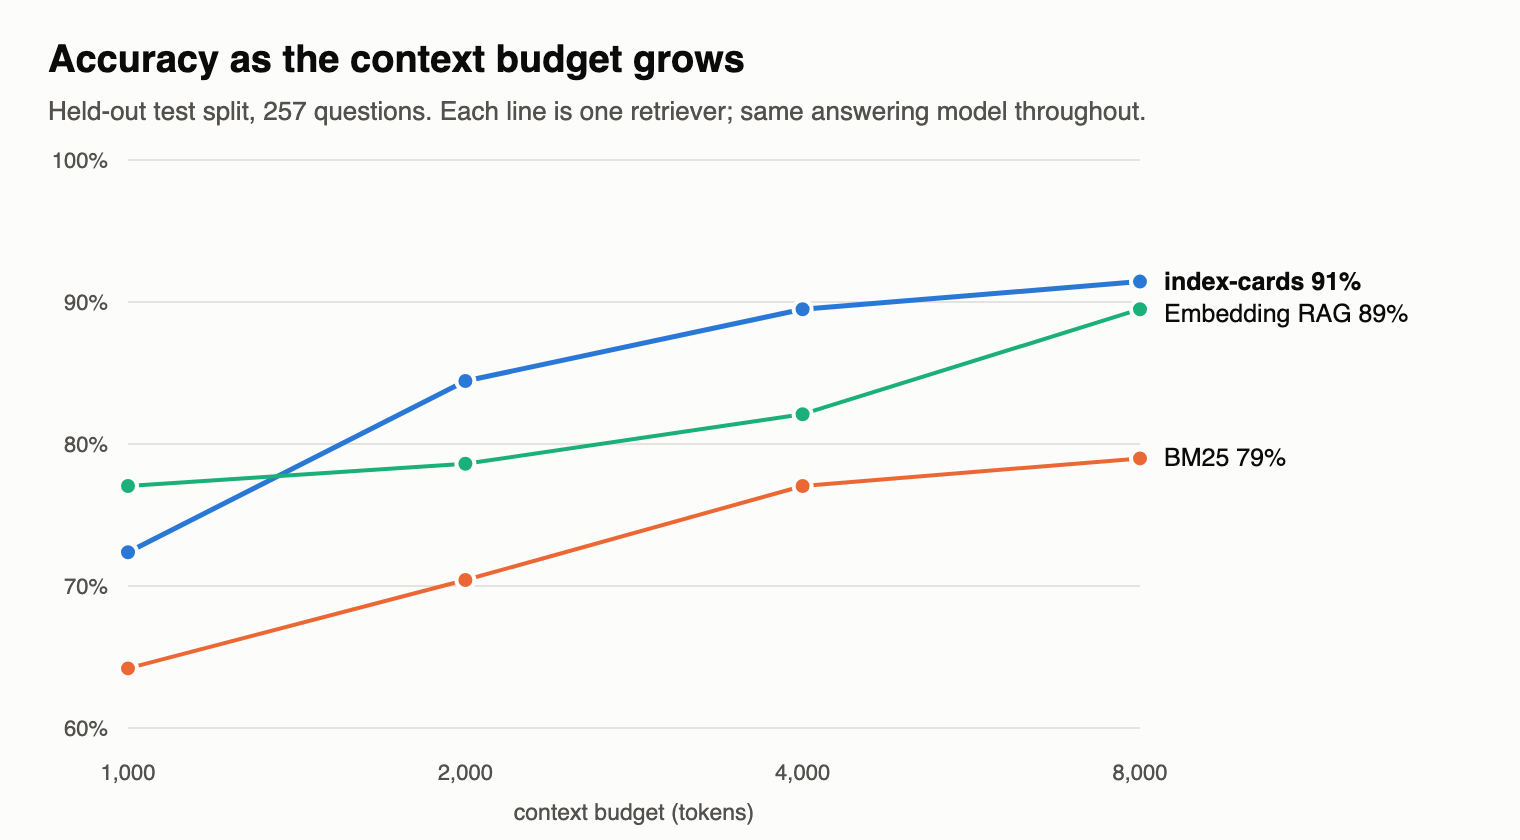
\includegraphics[width=0.85\linewidth]{figs/budget-sweep.png}
\caption{Accuracy against context budget on seed 8 (test split), Sonnet answering.}\label{fig:sweep}
\end{figure}

\textbf{Budget.} Figure~\ref{fig:sweep} varies $B$, and the advantage has a range. At 1{,}000 tokens RAG is ahead
(\MainRagOneAcc\% against \MainCardsOneAcc\%): a card's header, Timeline lines and defining note use most of a
small budget. At 2{,}000 and 4{,}000 tokens cards lead (\MainCardsTwoAcc\% against \MainRagTwoAcc\%, $p=\MainPRagTwo$;
and the 4{,}000 result above). At 8{,}000 tokens the two converge (\MainCardsEightAcc\% against \MainRagEightAcc\%,
$p=\MainPRagEight$), since RAG's window becomes large enough to hold both notes of a two-hop question. BM25 trails
throughout (\MainBmOneAcc\% to \MainBmEightAcc\%).

\section{The agent loop}\label{sec:agent}

\begin{table}[t]\centering\small
\caption{The agent loop: Claude Code with Read, Grep and Glob in the seed-7 vault, no budget, 91 test questions. Tokens are input tokens per question.}\label{tab:agent}
\begin{tabular}{lrrrrrr}\toprule
& \multicolumn{3}{c}{Sonnet} & \multicolumn{3}{c}{Haiku} \\
\cmidrule(lr){2-4}\cmidrule(lr){5-7}
Setup & Acc. & Tokens & Turns & Acc. & Tokens & Turns \\
\midrule
Vault only & 98.9 & 20{,}860 & 3.9 & 97.8 & 24{,}641 & 4.6 \\
Vault + memory file & 98.9 & 54{,}544 & 4.2 & 95.6 & 51{,}540 & 4.0 \\
Vault + index-cards & 97.8 & 26{,}211 & 5.4 & 89.0 & 45{,}439 & 6.9 \\
\bottomrule\end{tabular}\end{table}


Budgeted retrieval is one way an agent gets memory. The other is to let the agent search. We gave Claude Code Read,
Grep and Glob in a copy of the seed-7 vault, no budget and up to 30 turns, under three setups: the vault alone; the
vault with the memory file in the system prompt, as Claude Code loads \texttt{MEMORY.md}; and the vault with cards
plus the one-sentence pointer from the README (Table~\ref{tab:agent}).

Sonnet answers \AgSPlainAcc\% from the bare vault with \AgSPlainTok{} input tokens per question; cards add tokens
(\AgSCardsTok) and turns and do not add accuracy (\AgSCardsAcc\%). The memory file doubles the tokens. Haiku does
worse with cards (\AgHCardsAcc\% against \AgHPlainAcc\%): most of its extra misses answer ``where did I first meet
X?'' with a date. On a clean vault of this size, a model that can grep freely finds the answer itself, and the index
is overhead. Cards earn their place when context is a fixed budget: a hook that injects context, a prompt prefix,
a small model, a single retrieval call.

\section{Limitations}

The vaults are synthetic. A model wrote their prose from fact templates, so they are more regular than real notes,
every entity has a distinct name, and no one is referred to only by pronoun or role. Real vaults are larger and
messier, which may favour either side: grep and similarity have more noise to wade through, and cards have more
aliases to miss. The author of index-cards also built the benchmark; we report each category separately and log
every change made after seeing results. A few projects keep receiving status mentions after they were marked
cancelled or paused, which makes a handful of status questions ambiguous for every system. The memory baseline
simulates Claude Code's auto memory under the same budget and is not the product. The agent loop used one vault and
91 questions.

\section{Conclusion}

A deterministic entity index is a cheap, inspectable memory layer that matches similarity retrieval on single facts
and updates and clearly beats it on questions that need two notes, replicated on a world used once. Stale facts,
the usual worry, were rarely the failure once chunks carry dates; missing notes were. When the agent can search for
itself without a budget, the index adds cost without adding accuracy. Everything needed to rerun these numbers is in
the repository.

\begin{thebibliography}{9}\small
\bibitem{longmemeval} D.~Wu et al. LongMemEval: Benchmarking chat assistants on long-term interactive memory. arXiv:2410.10813, 2024.
\bibitem{mastra} Mastra. Yes, you can use RAG for agent memory. \url{https://mastra.ai/research/use-rag-for-agent-memory}, 2025.
\bibitem{melt} Shisa.AI. MELT: Testing long-lived memory for agentic AI. \url{https://blog.shisa.ai/posts/melt/}, 2026.
\bibitem{mom} MoM: Memory of memory. arXiv:2609.25054, 2026.
\bibitem{ccmemory} Anthropic. Claude Code documentation: memory. \url{https://docs.claude.com/en/docs/claude-code/memory}, 2026.
\bibitem{amb} AMB: an open, preregistered benchmark for memory layers in coding agents. \url{https://discuss.huggingface.co/t/179762}, 2026.
\end{thebibliography}

\end{document}
